\documentclass[11pt,a4paper]{article}
\usepackage[margin=2.5cm]{geometry}
\usepackage{amsmath,amssymb}
\usepackage{enumitem}
\usepackage{graphicx}
\usepackage{booktabs}
\usepackage[hidelinks]{hyperref}

% figures are written by the pipeline to outputs/ at the top of the repository
\graphicspath{{../outputs/}{outputs/}}

\newcommand{\given}{\,|\,}
\newcommand{\bin}{\operatorname{binomial}}
\newcommand{\pois}{\operatorname{Poisson}}
\newcommand{\nb}{\operatorname{NB}}

\title{Bundibugyo virus disease, 2026: estimates from a model in which $R_t$
and the reporting delay change at unknown times}
\author{}
\date{\today}

\begin{document}
\maketitle

This note describes the model fitted to confirmed cases of Bundibugyo virus
disease and gives its results as of the situation report of 1 October 2026.
The notation is that of Bajaj, Thompson and Lambert \cite{bajaj2025}.

\section{Data}

Each situation report gives the number of confirmed cases by date of symptom
onset. Write $C(t\given t')$ for the number with onset on day $t$ shown in the
report of day $t'$. There are 44 reports, from 12 July to 1 October 2026.
Onset days from 12 July, the date of the first report, are analysed (82
days). For earlier onset days nothing is known of reporting in the weeks after
onset, so they tell us nothing about the reporting delay and their reporting
is not modelled. Their counts are still used: the counts for the 40 days
before 12 July, as given in the report of the analysis date, enter the
transmission model as known earlier cases (\S\ref{sec:transmission}).

\paragraph{The correction of 6 September.} The report of 6 September removed
119 cases from 18 onset days between 14 May and 22 June. All of these onset
days are before 12 July, so this removal is not among the reported counts
which are modelled, and no special provision is made for it. It affects the
analysis only through the known earlier cases: analyses dated before 6
September use the counts as they stood before the removal (1750 cases in the
40 days before 12 July, against 1674 afterwards). Among the onset days which
are modelled, the largest fall in a count between two reports is of 2
cases.

\section{Model}\label{sec:model}

\subsection{Transmission}\label{sec:transmission}

$I(t)$ is the true number of cases with onset on day $t$, which is unknown.
Given earlier cases it follows the renewal equation with overdispersion,
\begin{equation}\label{eq:renewal}
I(t)\sim\nb\bigl(R_t\,\Lambda_t,\;\kappa\bigr),\qquad
\Lambda_t=\sum_{s=1}^{40}\omega_s\,I(t-s),
\end{equation}
a negative binomial distribution with mean $R_t\Lambda_t$ and variance
$R_t\Lambda_t(1+R_t\Lambda_t/\kappa)$.

\paragraph{Serial interval.} The weights $\omega_s$ are a discrete version of
a gamma serial interval with mean 15.3 and standard deviation 9.3 days, the
values estimated for Zaire ebolavirus in West Africa \cite{who2014}, there
being no published estimate for Bundibugyo virus. The weight for an interval
of $s$ days is the probability which the gamma distribution gives to
$(s-\tfrac12,\,s+\tfrac12)$, for $s=1,\dots,40$, rescaled to sum to one.
Cutting the distribution off at 40 days removes 1.8\% of its mass; as used,
the serial interval has mean 14.7 and standard deviation 8.2 days. There is
more than one way to make a continuous serial interval discrete, and the
choice matters most when the serial interval is short relative to a day,
which is not the case here: an alternative in common use \cite{cori2013}
allows for onset at any time within the day for both the infector and the
person infected, which spreads each weight over neighbouring days. The same
weights are used in every part of the fitting.

\paragraph{Cases before the first onset day analysed.} For the first 40 onset
days analysed, $\Lambda_t$ involves cases with onset before 12 July. These
are supplied as known: $I(t)$ for $t\le 0$ is set to the count in the report
of the analysis date, and is not estimated. By the analysis date these onset
days are at least five weeks old, so their counts are close to complete. No
model of how they came to be reported is needed for this, since they enter
only through $\Lambda_t$. Without them, $\Lambda_t$ would be understated for
the first weeks and $R_t$ overstated.

\subsection{Changes in $R_t$}\label{sec:Rt}

$R_t$ is piecewise constant. Onset days $1,\dots,T$ (here $T=82$) are divided
into $K_R+1$ segments which start on days $1=\tau_0<\tau_1<\dots<\tau_{K_R}$,
and $R_t=R_j$ for onset days in segment $j$. The number of changes $K_R$ and
the days $\tau_k$ are unknown.

\paragraph{Prior for the partition.} Each onset day after the first starts a
new segment with probability $p_R$, independently, and $p_R$ has a beta
prior:
\begin{equation}\label{eq:partitionprior}
p(\tau_1,\dots,\tau_{K}\given p_R) \propto p_R^{K}(1-p_R)^{T-1-K},
\qquad p_R\sim\operatorname{beta}(a,b),
\end{equation}
for partitions in which every segment has at least $\ell$ days, and zero
otherwise.
With $p_R$ integrated out, the prior probability of a partition depends only
on its number of changes,
\begin{equation}\label{eq:partitionmarginal}
p(\tau_1,\dots,\tau_K) \propto B(a+K,\,b+T-1-K)
\end{equation}
for the same partitions, where $B$ is the beta function. We take $a=1$, $b=T$ and $\ell=7$.

\paragraph{Implied prior on the number of changes.} Equation
\eqref{eq:partitionmarginal} is the weight of a \emph{single} partition, that
is, of one particular set of days on which changes occur. It falls steeply
with the number of changes: with $a=1$, $b=T=82$ it is $1/163$ for the one
partition with no change and $1/(163\times 162)$ for each partition with one
change. This does not mean that almost all prior probability is on $K=0$,
because the number of partitions with $k$ changes grows almost as quickly. The
prior probability of $k$ changes is the weight of one such partition
multiplied by the number of them, $N_\ell(k)$:
\begin{equation}\label{eq:priorK}
\Pr(K=k)=\frac{N_\ell(k)\,B(a+k,\,b+T-1-k)}
{\sum_{j\ge 0}N_\ell(j)\,B(a+j,\,b+T-1-j)}.
\end{equation}
\begin{itemize}[itemsep=2pt]
\item \emph{Without a minimum length} ($\ell=1$), a change can occur on any of
the $T-1$ days after the first, so $N_1(k)=\binom{T-1}{k}$, the denominator
is $B(a,b)$ and $K$ is beta-binomial:
\begin{align}
\Pr(K=k)&=\binom{T-1}{k}\frac{B(a+k,\,b+T-1-k)}{B(a,b)}, \label{eq:betabinomial}\\
\Pr(K=0)&=\frac{B(a,\,b+T-1)}{B(a,b)}=\frac{b}{b+T-1}\quad\text{when } a=1.
\end{align}
With $b=T=82$ this gives $\Pr(K=0)=82/163=0.50$ and a mean of
$(T-1)a/(a+b)=0.98$ changes.
\item \emph{With a minimum length of $\ell$ days}, as fitted, the weight of
each allowed partition is unchanged but fewer are allowed. The number of ways
of dividing $T$ days into $k+1$ segments of at least $\ell$ days each is
\begin{equation}\label{eq:countvalid}
N_\ell(k)=\binom{T-\ell(k+1)+k}{k},
\end{equation}
and zero if $T<\ell(k+1)$, so that at most 10 changes are possible here. Since
$N_\ell(k)<N_1(k)$ for $k\ge 1$, by more for larger $k$, probability moves
towards fewer changes.
\end{itemize}
The two priors are

\begin{center}
\begin{tabular}{lccccc}
\toprule
Number of changes & 0 & 1 & 2 & 3 & 4 or more \\
\midrule
No minimum length & 0.50 & 0.25 & 0.13 & 0.06 & 0.06 \\
Minimum of 7 days (as fitted) & 0.61 & 0.26 & 0.09 & 0.03 & 0.01 \\
\bottomrule
\end{tabular}
\end{center}

\noindent with a mean of 0.55 changes. The prior therefore favours no change,
and since $p_R$ is learned the penalty for a further change adapts to the
number already supported. The minimum length
prevents a segment being fitted to the last few onset days, for which little
has yet been reported.

Given $p_R$, \eqref{eq:partitionprior} is a product partition model for
change points in the sense of Barry and Hartigan \cite{barry1992}: the
probability of a partition is a product of a term for each segment, here
$p_R(1-p_R)^{n-1}$ for a segment of $n\ge\ell$ days (without the leading
$p_R$ for the first). Placing a prior on the probability of a change follows
\cite{barry1993}. It plays the role of the Pitman--Yor process prior used for
$R_t$ by \cite{creswell2022}, with a simpler form.

\paragraph{Prior for the values.} $R_j\sim\operatorname{gamma}(1,1)$
independently (shape and rate).

\subsection{Reporting}

A case with onset on day $t$ is reported after a delay which has a gamma
distribution with mean $\mu$ and standard deviation $\sigma$. Write
$\theta=(\mu,\sigma)$ and $S_\theta(t\given t')$ for the probability that the
case has not been reported by the end of day $t'$. Days are whole, and onset
is taken to occur at the middle of day $t$, so that with $G_\theta$ the
distribution function of the gamma delay,
\begin{equation}\label{eq:S}
S_\theta(t\given t')=1-G_\theta\bigl(t'-t+\tfrac12\bigr),\qquad t'\ge t.
\end{equation}
In particular $S_\theta(t\given t)=1-G_\theta(\tfrac12)$ is not one: it is
the probability that a case is not reported within the half day which remains
of its onset day. It is close to one (about 0.99 for the delays estimated
here). It cancels from the probability that a genuine case is newly reported,
$p_j(t)$ below, which involves only ratios of $S_\theta$, and enters the rate
at which erroneous records are added only as this factor.

\paragraph{Day of the week.} Reporting is assumed to be faster or slower according to the
day of the week on which a report is made. This is expressed through the
daily hazard of reporting. For a case with onset on day $t$ which is still
unreported at the end of day $k-1$, the hazard on day $k$ under the gamma
delay alone is
\begin{equation}\label{eq:hazard}
h_\theta(t,k)=\log S_\theta(t\given k-1)-\log S_\theta(t\given k),
\end{equation}
so that $S_\theta(t\given t')=S_\theta(t\given t)\exp\{-\sum_{k=t+1}^{t'}h_\theta(t,k)\}$.
Each day's hazard is multiplied by a factor $m_k$, giving
\begin{equation}\label{eq:Seffective}
S^{*}_\theta(t\given t') = S_\theta(t\given t)\,
\exp\Bigl\{-\sum_{k=t+1}^{t'} m_k\,h_\theta(t,k)\Bigr\},
\end{equation}
which is a proper survival function for any positive $m_k$, and is $S_\theta$
when every $m_k=1$.

It remains to say what $m_k$ is. There are seven parameters
$\psi_{\text{Mon}},\dots,\psi_{\text{Sun}}$, one for each day of the week on
which a situation report can be published. Situation reports are not
published every day. For each calendar day $k$, find the first situation
report published on day $k$ or later; this is the report in which a case
reported on day $k$ first appears. Then $m_k$ is the parameter $\psi$ for the
day of the week on which \emph{that report} was published. In symbols, if
$r(k)$ is the day on which that report was published and $w(\cdot)$ gives the
day of the week of a day,
\begin{equation}\label{eq:multiplier}
m_k=\psi_{w(r(k))}.
\end{equation}

\emph{Example.} Suppose one situation report is published on a Friday, none
on the Saturday or the Sunday, and the next on the Monday.

\begin{center}
\begin{tabular}{lcccc}
\toprule
Calendar day $k$ & Friday & Saturday & Sunday & Monday \\
\midrule
Report published on day $k$? & yes & no & no & yes \\
First report on or after day $k$ & Friday's & Monday's & Monday's & Monday's \\
$m_k$ & $\psi_{\text{Fri}}$ & $\psi_{\text{Mon}}$ & $\psi_{\text{Mon}}$ & $\psi_{\text{Mon}}$ \\
\bottomrule
\end{tabular}
\end{center}

\noindent A case reported on the Friday appears in Friday's report, so the
hazard of reporting on the Friday is multiplied by $\psi_{\text{Fri}}$. A case
reported on the Saturday, the Sunday or the Monday appears for the first time
in Monday's report, so the hazards of all three of those days are multiplied
by $\psi_{\text{Mon}}$. The parameters $\psi_{\text{Sat}}$ and
$\psi_{\text{Sun}}$ are not used here, because no report was published on
those days.

The reason for this construction is that the data show only how many cases
were added between Friday's report and Monday's report, and not on which of
the three days each was reported. By \eqref{eq:Seffective}, the probability
that a case with onset on day $t$, absent from Friday's report, appears in
Monday's is
\begin{equation}\label{eq:example}
1-\exp\bigl\{-\psi_{\text{Mon}}\,
[h_\theta(t,\text{Sat})+h_\theta(t,\text{Sun})+h_\theta(t,\text{Mon})]\bigr\}.
\end{equation}
With $\psi_{\text{Mon}}=1$ this is what the gamma delay alone gives. With
$\psi_{\text{Mon}}=1.2$, say, the hazard over the three days is 20\% higher,
and Monday reports contain more newly reported cases than the gamma delay
alone would give; with $\psi_{\text{Mon}}<1$ they contain fewer.

The $\psi_w$ are constrained by $\sum_w\log\psi_w=0$, so that they describe
differences between days of the week and not the overall speed of reporting,
which is the role of $\theta$. The six free $\log\psi_w$ have independent
$N(0,1)$ priors. The $\psi_w$ do not depend on the onset day, and are shared
by all segments of the delay described next.

\paragraph{Changes in the delay.} $\theta$ is assumed piecewise constant over onset
days: a case's delay distribution depends on its onset day. The segments have
the same form of prior as those of $R_t$, \eqref{eq:partitionprior} with
$a=1$, $b=T$ and $\ell=7$, and are independent of them, with their own
probability of a change. The values $\theta_j=(\mu_j,\sigma_j)$ of the
segments are tied together by a hierarchical prior:
\begin{equation}\label{eq:delayhierarchy}
\log\mu_j\sim N(\log\mu_0,\,s^2),\qquad \log\sigma_j\sim N(\log\sigma_0,\,s^2),
\end{equation}
with $\mu_0\sim\operatorname{gamma}$ (mean 7, standard deviation 10 days),
$\sigma_0\sim\operatorname{gamma}$ (mean 5, standard deviation 5 days) and
$s\sim N^{+}(0,\,0.5^2)$, a normal distribution restricted to positive values.
Here $\mu_0$ and $\sigma_0$ are the mean and standard deviation of the delay
in a typical segment, and $s$ is a single unknown number which says how much
the segments differ from one another: it is the standard deviation, across
segments, of $\log\mu_j$ and of $\log\sigma_j$. A value of $s=0.2$, for
example, means that the mean delay of a segment is typically within about
20\% of $\mu_0$; $s$ near zero means that the segments have almost the same
delay.

\paragraph{Reported counts.} The count shown for an onset day is made up of
genuine cases and, occasionally, of records entered in error (for example a
duplicate, or a case later reclassified) which are subsequently removed.
Between consecutive reports on days $t_{j-1}$ and $t_j$, the count for onset
day $t$ changes through three independent quantities:
\begin{itemize}[itemsep=2pt]
\item $d_j(t)$, the number of genuine cases reported for the first time;
\item $n_j(t)$, the number of erroneous records added to the count;
\item $e_j(t)$, the number of erroneous records, added earlier, which are
removed from the count.
\end{itemize}
Their distributions are
\begin{align}
d_j(t) &\sim \bin\bigl(I(t) - D(t\given t_{j-1}),\; p_j(t)\bigr), \label{eq:d}\\
n_j(t) &\sim \pois\bigl(\eta\,I(t)\,[S^{*}_\theta(t\given t_{j-1}) - S^{*}_\theta(t\given t_j)]\bigr), \label{eq:n}\\
e_j(t) &\sim \bin\bigl(E(t\given t_{j-1}),\; 1-(1-\rho)^{\,t_j-t_{j-1}}\bigr), \label{eq:m}
\end{align}
where $p_j(t)=1-S^{*}_\theta(t\given t_j)/S^{*}_\theta(t\given t_{j-1})$,
$D$ is the number of genuine cases reported so far and $E$ the number of
erroneous records currently in the count, so that
\begin{equation}\label{eq:deltaC}
C(t\given t_j)-C(t\given t_{j-1}) = d_j(t)+n_j(t)-e_j(t).
\end{equation}
The form of \eqref{eq:n} reflects the assumption that erroneous records are a
by-product of reporting: whenever cases of an onset day are being reported,
each has a small chance of being accompanied by a record made in error. The
expected number of genuine cases reported in the interval is
$I(t)\,[S^{*}_\theta(t\given t_{j-1})-S^{*}_\theta(t\given t_j)]$, and
$\eta$ times this is the expected number of erroneous records added. A
Poisson distribution is the natural one for a count of rare events arising
independently in this way, and it has the practical advantage that the number
of erroneous records in the count at any time is also Poisson, which keeps
the likelihood simple. The rate depends on the expected and not the realised
number of genuine reports, so that $n_j(t)$ and $d_j(t)$ are independent
given $I(t)$.

With $\eta=0$ this is the model of \cite{bajaj2025}, in which counts can only
rise. The erroneous records allow the occasional small falls seen in the data
(the largest, for these onset days, is of 2 cases). $\eta$ is the expected
number of erroneous records per genuine case reported, with a gamma prior of
mean and standard deviation 0.005; $\rho$ is the daily probability that an
erroneous record is removed, with a $\operatorname{beta}(1,4)$ prior.

$D$ and $E$ are not observed. Given $I(t)$ and the parameters, the likelihood
of the counts for onset day $t$, $L_t$, is obtained by a forward recursion
over the possible values of $E$ (at most 3 here), and onset days are
independent given the $I(t)$.

\subsection{Summary of unknowns and priors}

\begin{center}
\begin{tabular}{lll}
\toprule
Unknown & Meaning & Prior \\
\midrule
$I(t)$ & true cases with onset on day $t$ & renewal model \eqref{eq:renewal} \\
$\kappa$ & overdispersion of transmission & gamma, mean 20, s.d.\ 20 \\
$K_R$, $\tau$ & changes in $R_t$ & \eqref{eq:partitionprior}, $a=1$, $b=T$, $\ell=7$ \\
$R_j$ & $R_t$ in segment $j$ & gamma, shape 1, rate 1 \\
$K_\theta$, $\tau^\theta$ & changes in the delay & \eqref{eq:partitionprior}, $a=1$, $b=T$, $\ell=7$ \\
$\mu_j$, $\sigma_j$ & mean and s.d.\ of delay in segment $j$ & \eqref{eq:delayhierarchy} \\
$\mu_0$, $\sigma_0$ & centres of the delay parameters & gamma, means 7 and 5, s.d.\ 10 and 5 \\
$s$ & spread of the delay parameters & half-normal, s.d.\ 0.5 \\
$\psi_w$ & effect of day of the week of a report & $\log\psi_w\sim N(0,1)$, summing to zero \\
$\eta$ & erroneous records per genuine report & gamma, mean 0.005, s.d.\ 0.005 \\
$\rho$ & daily probability an erroneous record is removed & beta$(1,4)$ \\
\bottomrule
\end{tabular}
\end{center}

\subsection{Fitting}

The posterior is sampled by Markov chain Monte Carlo. Each iteration updates,
in turn:
\begin{enumerate}[itemsep=2pt]
\item \emph{Each $I(t)$}, drawn from its conditional distribution over
integers, which combines the renewal terms for day $t$ and for the 40 days
after it with the reporting likelihood $L_t$.
\item \emph{The segments of $R_t$ and their values}, drawn jointly and exactly
given the $I(t)$, $\kappa$ and $p_R$. With $R_j$ integrated out, each
possible segment of onset days $u$ to $v$ has a marginal likelihood $M(u,v)$;
under a Poisson model this has a closed form, and under the negative binomial
model used here it is calculated numerically over a grid of 400 values of
$R$ between 0.02 and 20. Given $p_R$ the weight of a partition is a product
over its segments, so the summed weight $F(v)$ of all partitions of days
$1,\dots,v$ satisfies
\begin{equation}\label{eq:partitionforward}
F(v)=\sum_{u}F(u-1)\,M(u,v)\,p_R^{\,[u>1]}(1-p_R)^{\,v-u},\qquad F(0)=1,
\end{equation}
the sum being over starts $u$ which leave the segment long enough. The
partition is drawn by sampling the start of the last segment with
probabilities proportional to the terms of $F(T)$, then the start of the
segment before it, and so on. Each $R_j$ is then drawn from its conditional
distribution on the grid, and $p_R$ from
$\operatorname{beta}(a+K_R,\,b+T-1-K_R)$. The number of segments, and so
the number of values $R_j$, does change from one iteration to the next. But
because the $R_j$ are integrated out before the partition is drawn, the
partition is drawn directly from its conditional distribution over all
partitions, of whatever number of segments, and the $R_j$ are then drawn given
it. Nothing is proposed and then accepted or rejected, so the reversible-jump
moves usually needed when the number of parameters changes are not required
for $R_t$.
\item \emph{The segments of the delay}, by Metropolis--Hastings moves, with
their probability of a change integrated out as in
\eqref{eq:partitionmarginal}: a random-walk update of $(\mu_j,\sigma_j)$ in
each segment; a move which either splits a segment in two (one part keeping
its parameters and the other taking new ones proposed log-normally about
them) or merges two neighbouring segments; a move which shifts a change by up
to three days; and a random-walk update of $(\mu_0,\sigma_0,s)$. A split of a
segment which can be split in $n$ ways, taking $K$ changes to $K+1$, is
accepted with probability $\min(1,A)$,
\begin{equation}\label{eq:splitratio}
A=\frac{\prod_t L_t(\theta^*)}{\prod_t L_t(\theta_j)}\times
\frac{B(a+K+1,\,b+T-2-K)}{B(a+K,\,b+T-1-K)}\times
\frac{p(\theta^*\given\mu_0,\sigma_0,s)}{q(\theta^*\given\theta_j)}\times n,
\end{equation}
the products being over the onset days which take the new parameters
$\theta^*$ and $q$ being the density from which these were proposed; a merge
is accepted with the reciprocal for the split which would reverse it.
\item \emph{$\kappa$, the $\psi_w$, and $(\eta,\rho)$}, each by random-walk
Metropolis.
\end{enumerate}
The split-or-merge and shift moves of step 3 are each attempted five times in
every iteration, since they are cheap beside step 1.

For each analysis date three chains of 1500 iterations were run from
different starting values (of the true cases, the delay and $\kappa$), and
the first half of each discarded. Agreement between chains is measured by the
split-$\widehat R$ statistic, which compares the variation between the halves
of the chains with that within them; values close to 1 indicate agreement and
values above about 1.1 that the chains have not converged.

\paragraph{Checks of the software.} With no data, both samplers of segments
reproduce the prior \eqref{eq:partitionmarginal}; the exact draw of
partitions agrees with enumeration of all partitions of short series; and on
simulated data with two changes in each of $R_t$ and the delay, all four were
placed within three days of the truth with posterior probability one when
transmission was not overdispersed.

\section{Results as of 1 October 2026}

Results are from three chains pooled. Their agreement is examined in
\S\ref{sec:convergence}; in brief, the chains agree on the estimates of cases
and of $R_t$ but not on the number of changes in the delay.

\begin{figure}[h]
\centering
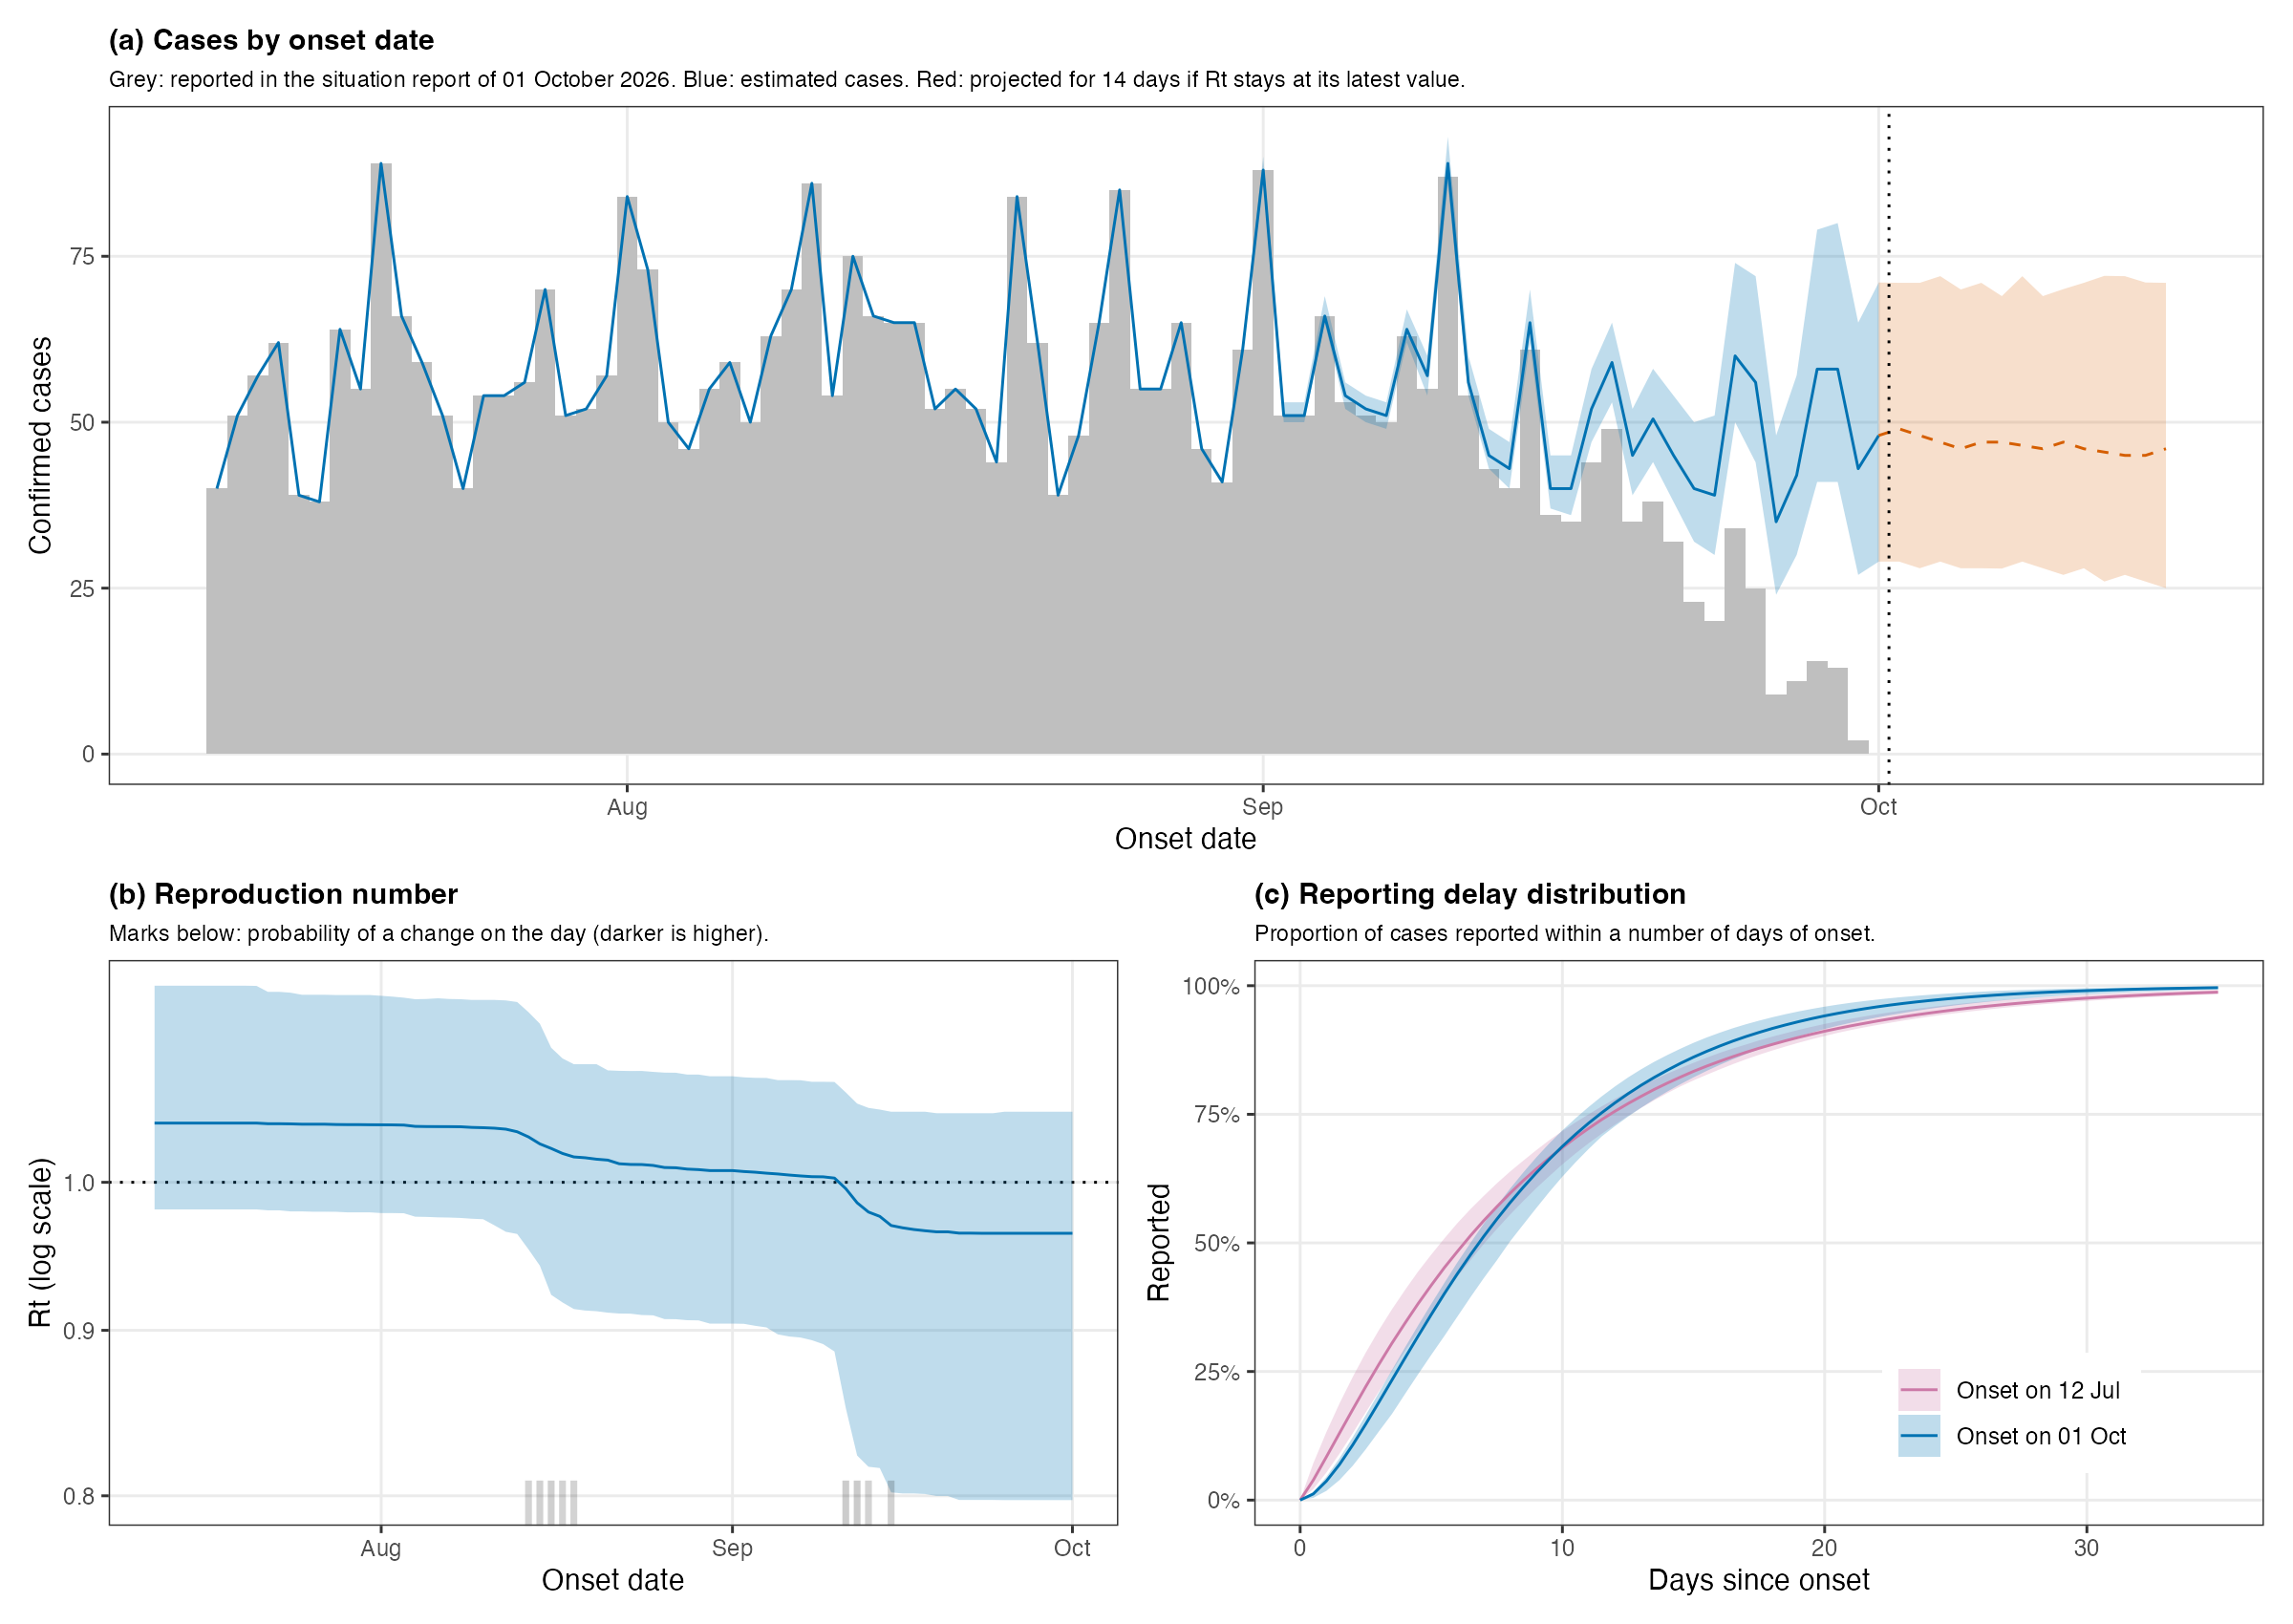
\includegraphics[width=\textwidth]{bvd_changepoint_main.png}
\caption{Estimates from the situation report of 1 October 2026. (a) Confirmed
cases by onset date: those reported (grey), the estimated true number (blue,
posterior median and 90\% interval) and a projection for 14 days if $R_t$
stays at its latest value (red). (b) $R_t$ on a log scale, with marks showing
the posterior probability of a change on each day. (c) The reporting delay
distribution for the earliest and latest onset days.}
\label{fig:main}
\end{figure}

\paragraph{Cases.} For onset days more than about three weeks before the
report, the estimated number of cases is the number reported. For the latest
two weeks the report is far from complete (figure~\ref{fig:parameters}b) and
the estimates are well above the reported counts: for the last few onset
days, of which under 15 cases a day have been reported, the estimates are
between 40 and 60 cases a day with 90\% intervals from about 25 to about 80.
The estimates give no indication that cases are falling, although the
reported counts fall steeply. The projection, which assumes that $R_t$ stays
as it is, has a median of about 47 cases a day and a 90\% interval of roughly
25 to 72.

\paragraph{Reproduction number.} $R_t$ is estimated at about 1.07 for onset
days in July and early August, and at 0.96 (90\% interval 0.80 to 1.05) for
the latest onset day. There is modest support for one change (the posterior
mean number of changes is 0.6), placed either in mid-August or around 10
September. $R_t$ is therefore close to one throughout, with some evidence of
a small decline, and neither slow growth nor slow decline is excluded at
present.

\paragraph{Reporting delay.} For the latest onset days the delay has mean 8.4
days (7.9 to 9.3) and standard deviation 6.4 days (5.7 to 7.1). The
distributions for the earliest and latest onset days differ only a little:
about half of cases are reported within a week of onset in both. The number
and position of changes in the delay are not well determined
(\S\ref{sec:convergence}).

\begin{figure}[h]
\centering
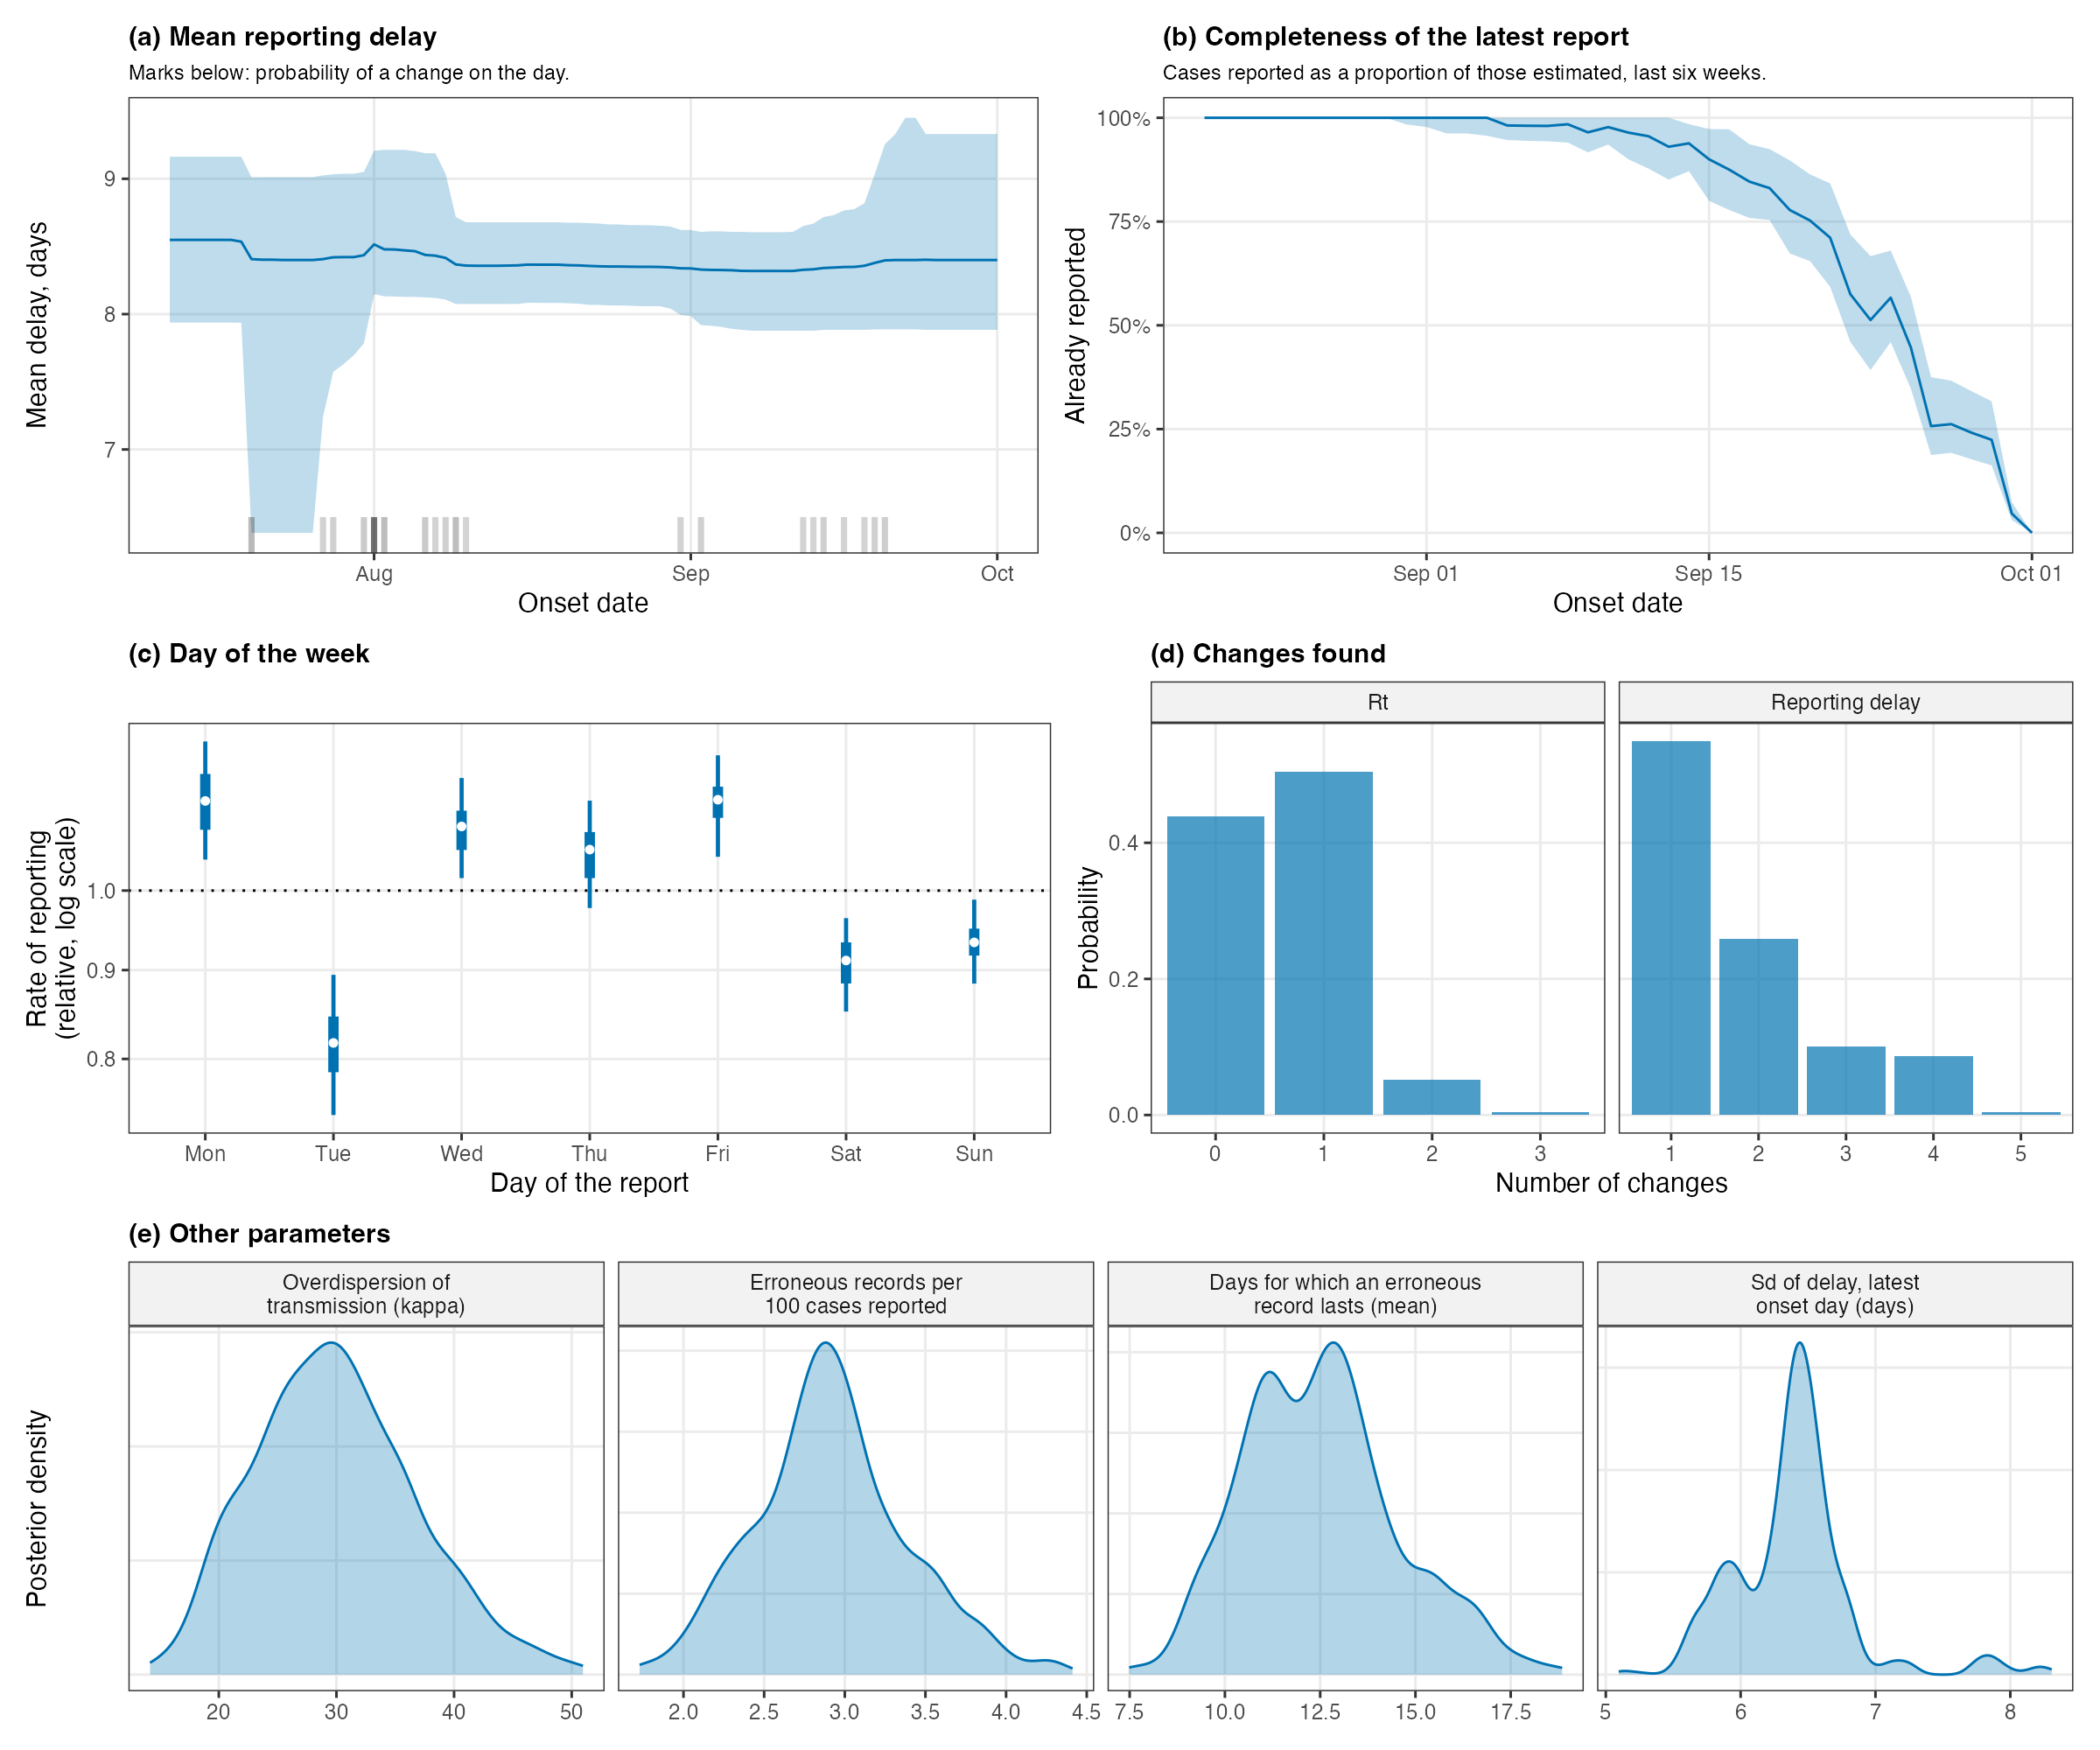
\includegraphics[width=\textwidth]{bvd_changepoint_parameters.png}
\caption{Further estimates from the situation report of 1 October 2026. (a)
Mean reporting delay by onset date. (b) Cases reported as a proportion of
those estimated, for the last six weeks. (c) Effect of the day of the week of
a report on the rate of reporting (median, 50\% and 90\% intervals). (d)
Posterior distribution of the number of changes in $R_t$ and in the delay. (e)
Posterior densities of the other parameters.}
\label{fig:parameters}
\end{figure}

\paragraph{Other parameters.}
\begin{itemize}[itemsep=2pt]
\item \emph{Day of the week.} Reports published on Mondays and Fridays contain
more newly reported cases than the delay alone would give
($\psi=1.13$ for both, 90\% intervals 1.04 to 1.22 and 1.05 to 1.20), as to a
lesser extent do those published on Wednesdays (1.09, 1.02 to 1.16). Those
published on Tuesdays contain fewer (0.82, 0.74 to 0.89), as do those on
Saturdays (0.91, 0.85 to 0.96) and Sundays (0.93, 0.88 to 0.99).
\item \emph{Overdispersion.} $\kappa=30$ (20 to 42): transmission is
moderately overdispersed. With 50 cases a day the variance of a day's cases
is about 2.7 times the mean.
\item \emph{Erroneous records.} About 3 are added per 100 genuine cases
reported ($\eta=0.029$, 0.022 to 0.038), and each is removed with probability
0.080 a day (0.061 to 0.106), so remains for about 12 days on average.
\end{itemize}

\section{Estimates made on earlier dates}

The same model was fitted to the reports available on five earlier dates, in
each case to onset days from 12 July and with the earlier cases as known on
that date, and its estimates compared with the counts in the report of 1
October (figure~\ref{fig:cases}, table~\ref{tab:dates}). Onset days in the two
weeks before 1 October are themselves incomplete in that report, so for the
analysis of 20 September the comparison is less secure than for the others.

\begin{figure}[h]
\centering
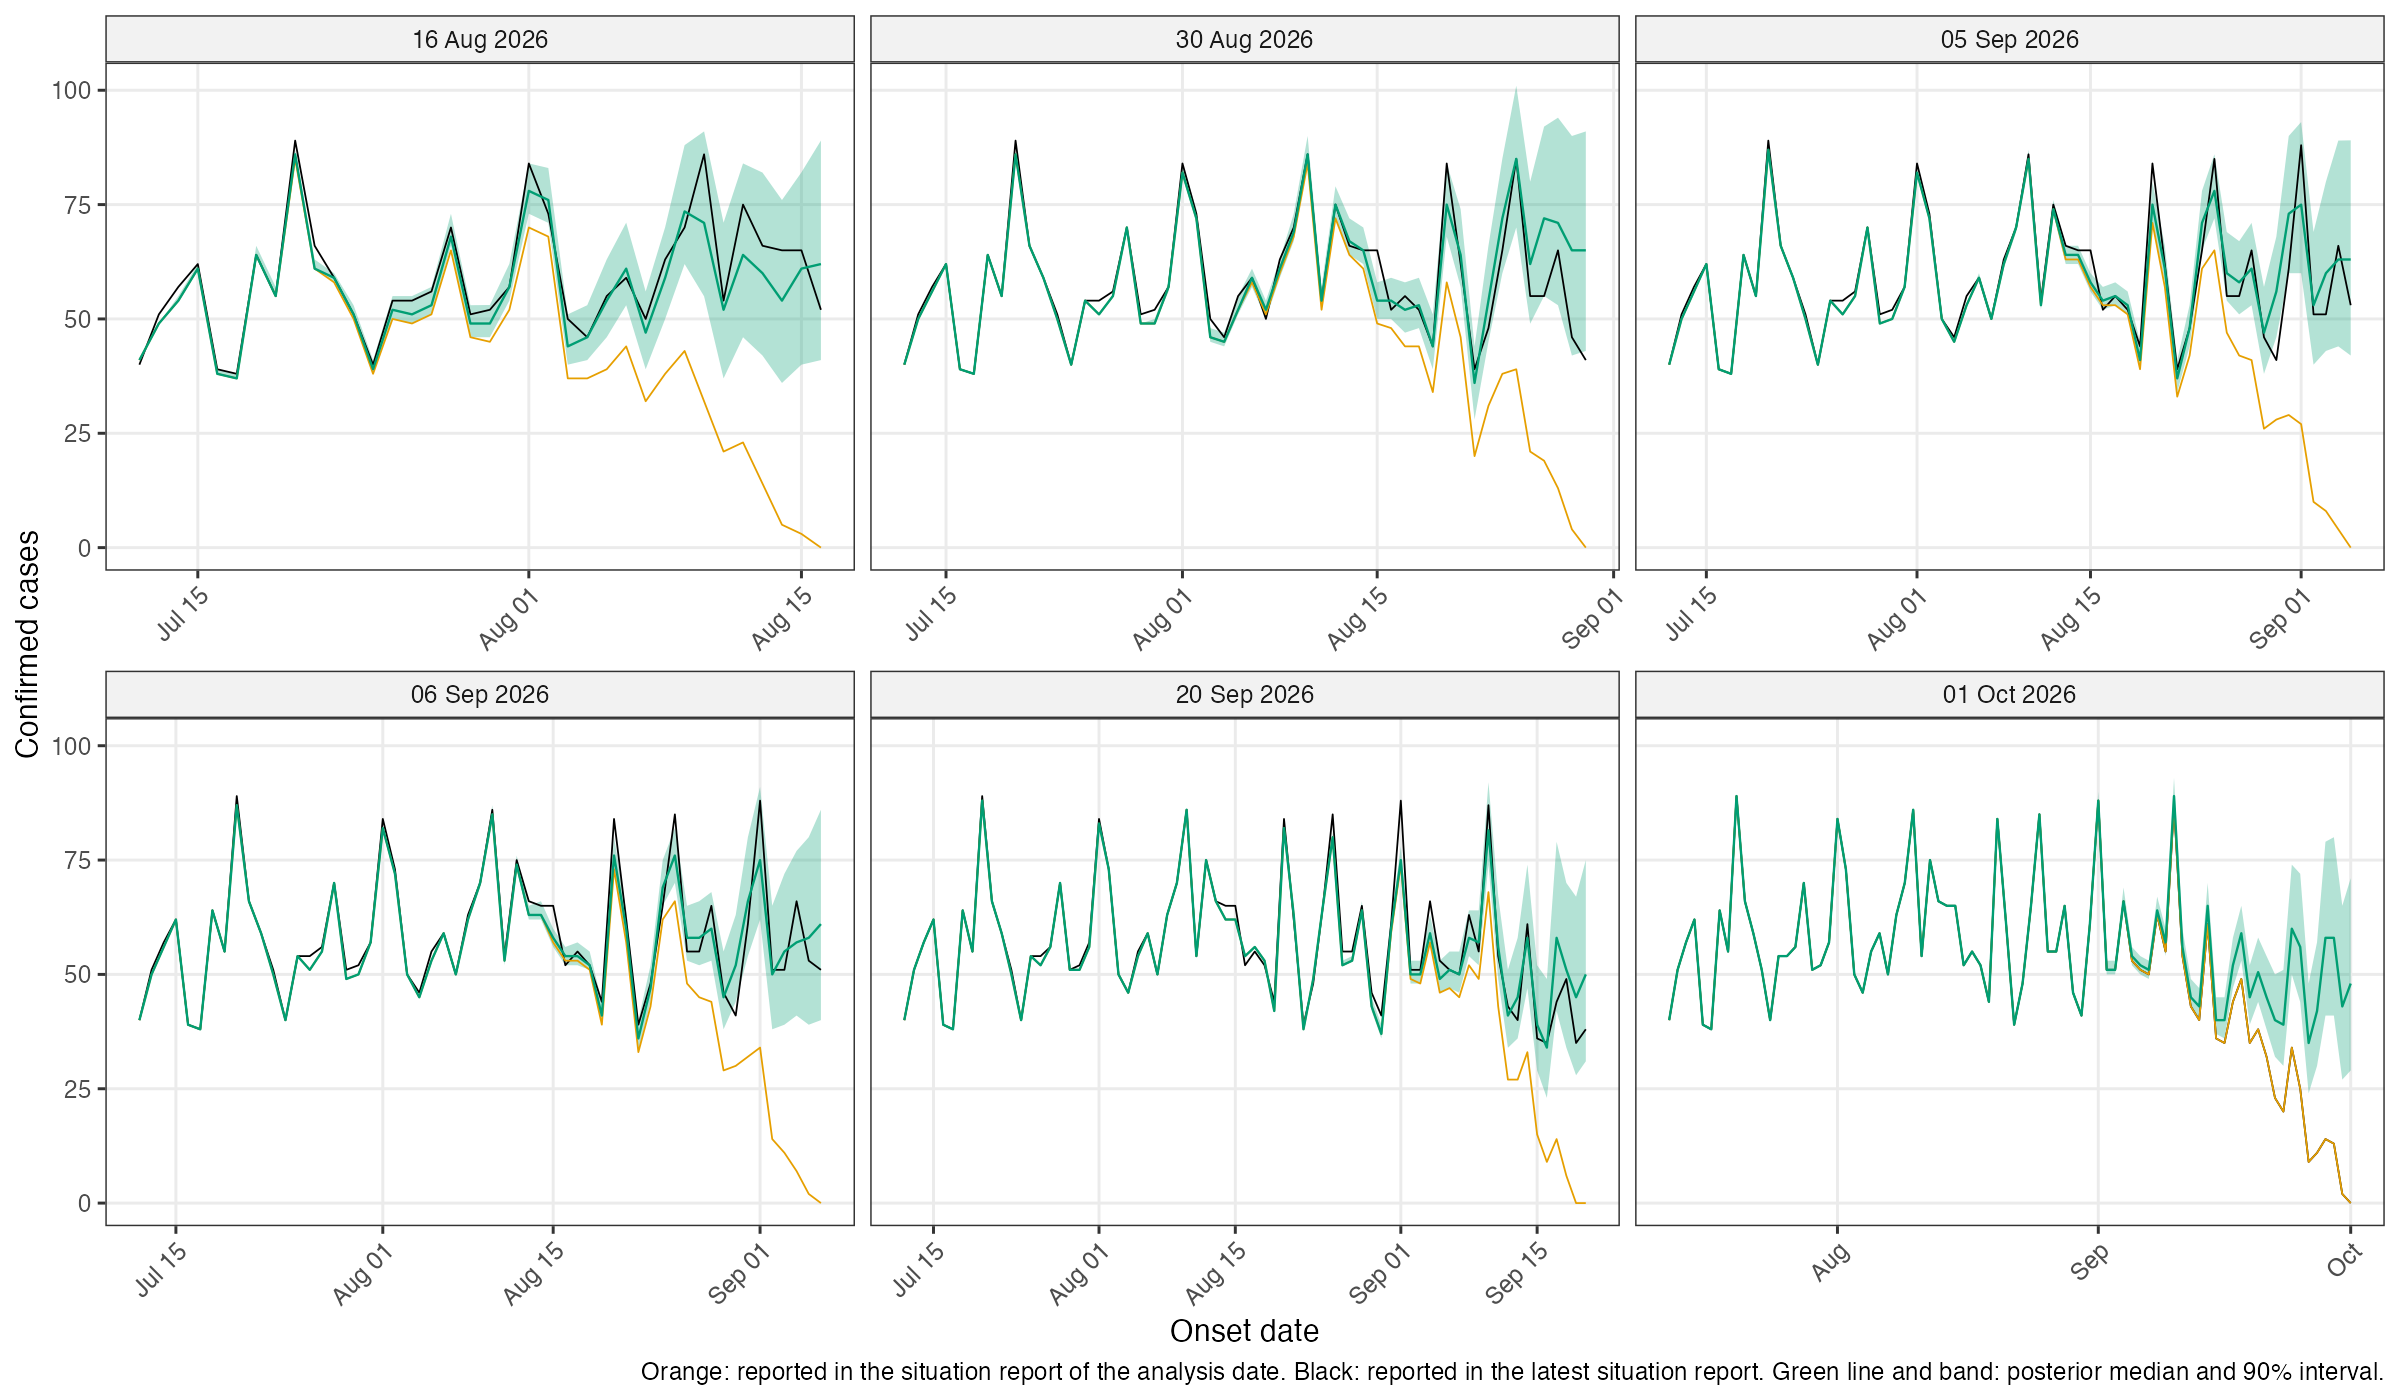
\includegraphics[width=\textwidth]{bvd_changepoint_cases.png}
\caption{Estimated cases by onset date as of each analysis date (green,
posterior median and 90\% interval), with the counts reported on that date
(orange) and in the report of 1 October (black).}
\label{fig:cases}
\end{figure}

\begin{table}[h]
\centering
\begin{tabular}{lccccc}
\toprule
Analysis date & Score & Coverage of & Bias & $R_t$, latest onset day & Mean delay, latest \\
 & & 90\% intervals & & & onset day (days) \\
\midrule
16 August & 0.056 & 100\% & $-6\%$ & 1.09 (1.01, 1.18) & 9.2 (8.3, 10.2) \\
30 August & 0.078 & 93\% & $+9\%$ & 1.08 (1.03, 1.16) & 8.7 (8.0, 9.2) \\
5 September & 0.066 & 93\% & $+4\%$ & 1.06 (1.01, 1.13) & 8.5 (7.9, 9.1) \\
6 September & 0.061 & 86\% & $+1\%$ & 1.06 (0.97, 1.11) & 8.4 (8.0, 8.8) \\
20 September & 0.060 & 100\% & $+5\%$ & 0.98 (0.72, 1.07) & 7.3 (6.8, 9.6) \\
1 October & & & & 0.96 (0.80, 1.05) & 8.4 (7.9, 9.3) \\
\bottomrule
\end{tabular}
\caption{Estimates for the latest 14 onset days on each analysis date,
compared with the counts in the report of 1 October. The score is the
weighted interval score relative to the mean count (smaller is better); the
bias is that of the posterior median relative to the mean count. Intervals
are 90\%.}
\label{tab:dates}
\end{table}

Estimates of recent counts made on each earlier date were close to what was
later reported: the 90\% intervals contained between 86\% and 100\% of the
later counts and the bias was at most 9\%. The estimate of $R_t$ for the
latest onset day was a little above one, with an interval excluding one,
until early September, and has since fallen to a little below one.

\section{Posterior predictive checks}

The model fitted on 1 October was checked by simulating from it. For each of
900 posterior draws:
\begin{itemize}[itemsep=2pt]
\item \emph{Reporting.} Given the draw's true cases, delay parameters, effects
of the day of the week, $\eta$ and $\rho$, reported counts were simulated for
every onset day and every report, and compared with the counts in the
situation reports.
\item \emph{Transmission.} Given the draw's $R_t$ and $\kappa$, the cases of
each onset day were simulated from \eqref{eq:renewal} given the cases before
it, and compared with the draw's own true cases.
\end{itemize}

\begin{figure}[h]
\centering
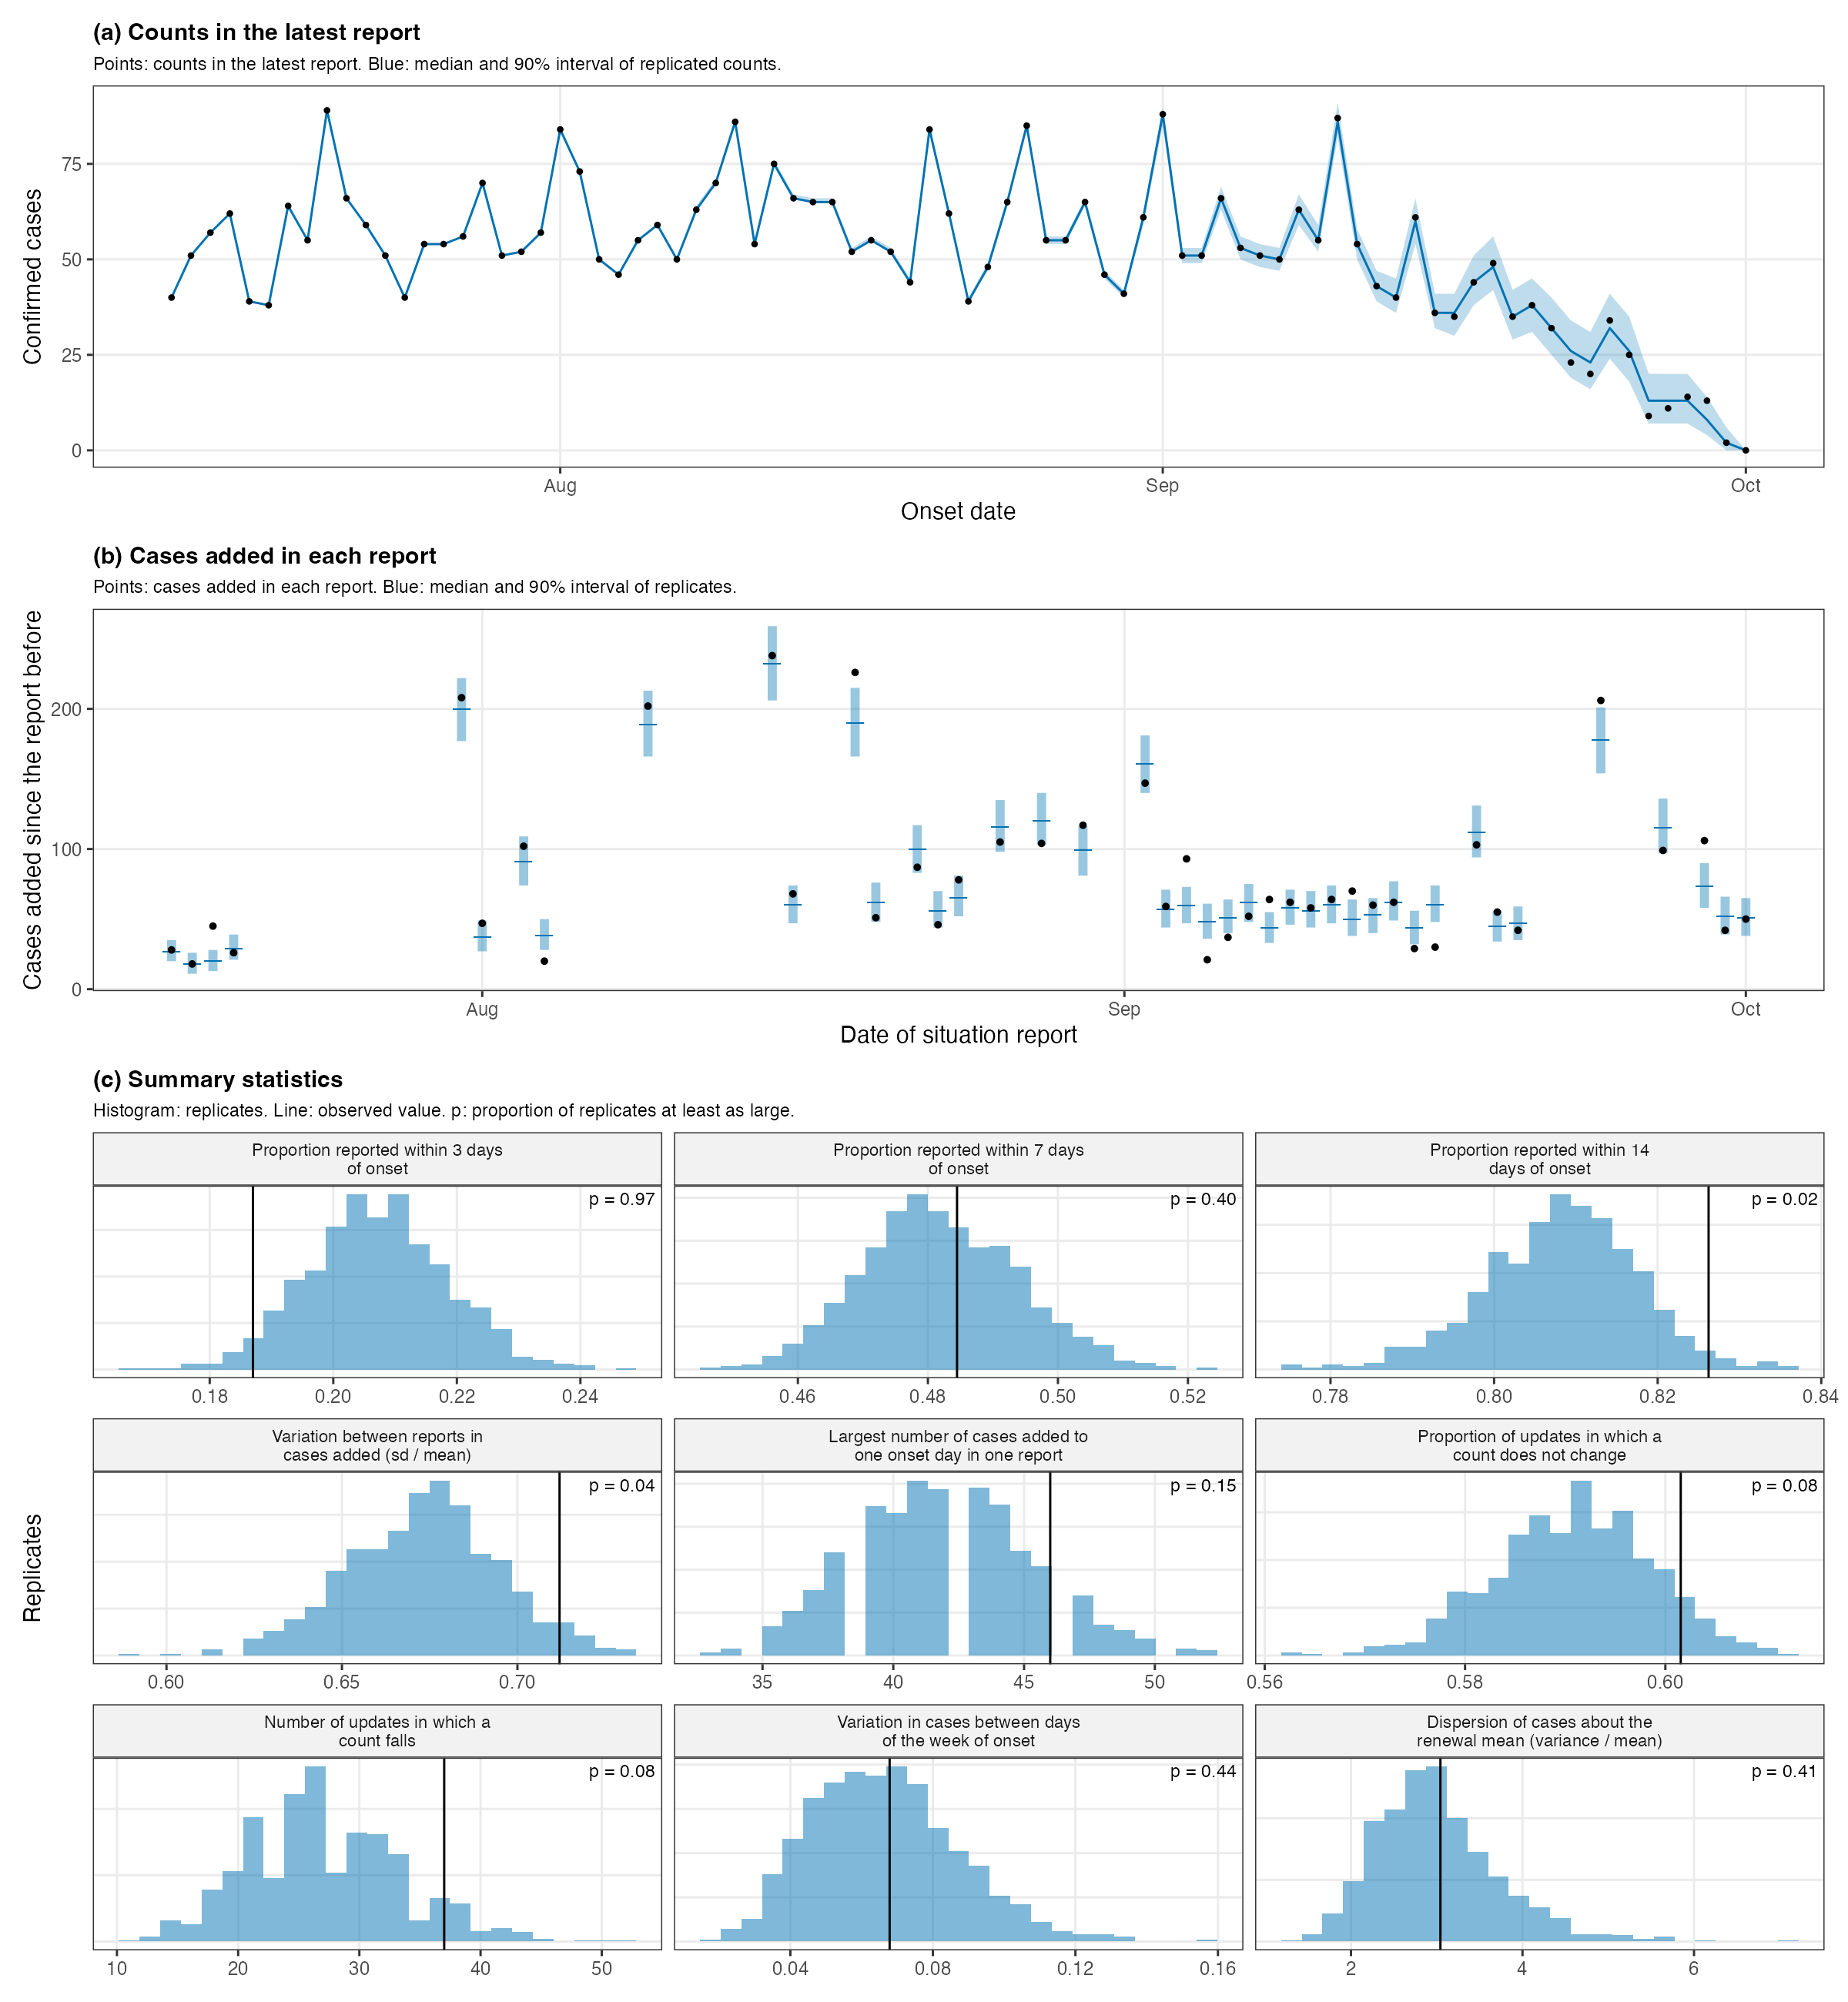
\includegraphics[width=0.95\textwidth]{bvd_changepoint_checks.png}
\caption{Posterior predictive checks. (a) Counts in the report of 1 October
(points) against replicated counts (blue, median and 90\% interval). (b) Cases
added in each report against the replicates. (c) Summary statistics: the
distribution over replicates, the observed value (line) and the proportion of
replicates at least as large ($p$).}
\label{fig:checks}
\end{figure}

\begin{table}[h]
\centering
\begin{tabular}{lccc}
\toprule
Statistic & Observed & Replicates (median, 90\% interval) & $p$ \\
\midrule
\emph{Reporting} \\
Proportion reported within 3 days of onset & 0.187 & 0.207 (0.189, 0.226) & 0.97 \\
Proportion reported within 7 days of onset & 0.485 & 0.481 (0.463, 0.502) & 0.40 \\
Proportion reported within 14 days of onset & 0.826 & 0.809 (0.792, 0.822) & 0.02 \\
Variation between reports in cases added (sd/mean) & 0.712 & 0.674 (0.637, 0.709) & 0.04 \\
Largest addition to one onset day in one report & 46 & 42 (36, 48) & 0.15 \\
Proportion of updates in which a count does not change & 0.602 & 0.591 (0.578, 0.603) & 0.08 \\
Number of updates in which a count falls & 37 & 26 (17, 38) & 0.08 \\
\addlinespace
\emph{Transmission} \\
Dispersion of cases about the renewal mean (variance/mean) & 3.0 & 2.9 (2.0, 4.3) & 0.41 \\
Variation in cases between days of the week of onset & 0.068 & 0.065 (0.036, 0.104) & 0.44 \\
\bottomrule
\end{tabular}
\caption{Posterior predictive checks. $p$ is the proportion of replicates at
least as large as the observed value; values near 0 or 1 indicate a feature
which the model does not reproduce. For transmission the observed value is
that of the true cases of each draw (the median is shown).}
\label{tab:checks}
\end{table}

\begin{itemize}[itemsep=2pt]
\item \emph{Transmission is described adequately.} The dispersion of cases
about the renewal mean is what the fitted model gives ($p=0.41$). The peaks
about a week apart in the counts by onset date (figure~\ref{fig:main}a) are
no more than the model produces by chance ($p=0.44$), so there is no need for
an effect of the day of the week of onset. In an earlier version of this
analysis, in which cases before 12 July were not supplied, the first of these
checks failed badly: the misfit at the start of the series was absorbed as
overdispersion ($\kappa$ of about 4).
\item \emph{Reporting is described adequately, with a small misfit in the
shape of the delay.} The cases added in each report are reproduced
(figure~\ref{fig:checks}b), including the large differences between reports
which follow from their spacing and day of the week. Slightly less is
reported within 3 days ($p=0.97$) and slightly more within 14 days
($p=0.02$) than the model gives, which suggests that the gamma shape is not
quite right, and the variation between reports is a little greater than the
model gives ($p=0.04$). None of these discrepancies is large.
\end{itemize}

\section{Convergence}\label{sec:convergence}

\begin{table}[h]
\centering
\begin{tabular}{lcccccc}
\toprule
 & \multicolumn{6}{c}{Analysis date} \\
Quantity & 16 Aug & 30 Aug & 5 Sep & 6 Sep & 20 Sep & 1 Oct \\
\midrule
$R_t$, latest onset day & 1.00 & 1.01 & 1.00 & 1.00 & 1.02 & 1.04 \\
Cases, latest 14 onset days in total & 1.02 & 1.01 & 1.03 & 1.02 & 1.08 & 1.05 \\
Cases, worst single onset day & 1.03 & 1.02 & 1.04 & 1.02 & 1.10 & 1.02 \\
Number of changes in $R_t$ & 1.00 & 1.00 & 1.01 & 1.00 & 1.01 & 1.03 \\
$\kappa$ & 1.28 & 1.08 & 1.06 & 1.05 & 1.03 & 1.05 \\
$\eta$ & 1.05 & 1.02 & 1.01 & 1.03 & 1.03 & 1.02 \\
$\rho$ & 1.05 & 1.01 & 1.01 & 1.00 & 1.00 & 1.03 \\
\addlinespace
Mean delay, latest onset day & 1.08 & 1.12 & 1.23 & 1.23 & 1.25 & 1.13 \\
Standard deviation of delay, latest onset day & 1.08 & 1.17 & 1.28 & 1.16 & 1.23 & 1.26 \\
Number of changes in delay & 1.03 & 1.03 & 1.04 & 1.19 & 1.46 & 1.57 \\
Effects of day of week (worst) & 1.08 & 1.45 & 1.20 & 1.87 & 1.10 & 1.15 \\
\bottomrule
\end{tabular}
\caption{Split-$\widehat R$ from three chains of 1500 iterations for each
analysis date. Values above about 1.1 indicate that the chains have not
converged for that quantity.}
\label{tab:rhat}
\end{table}

\begin{figure}[h]
\centering
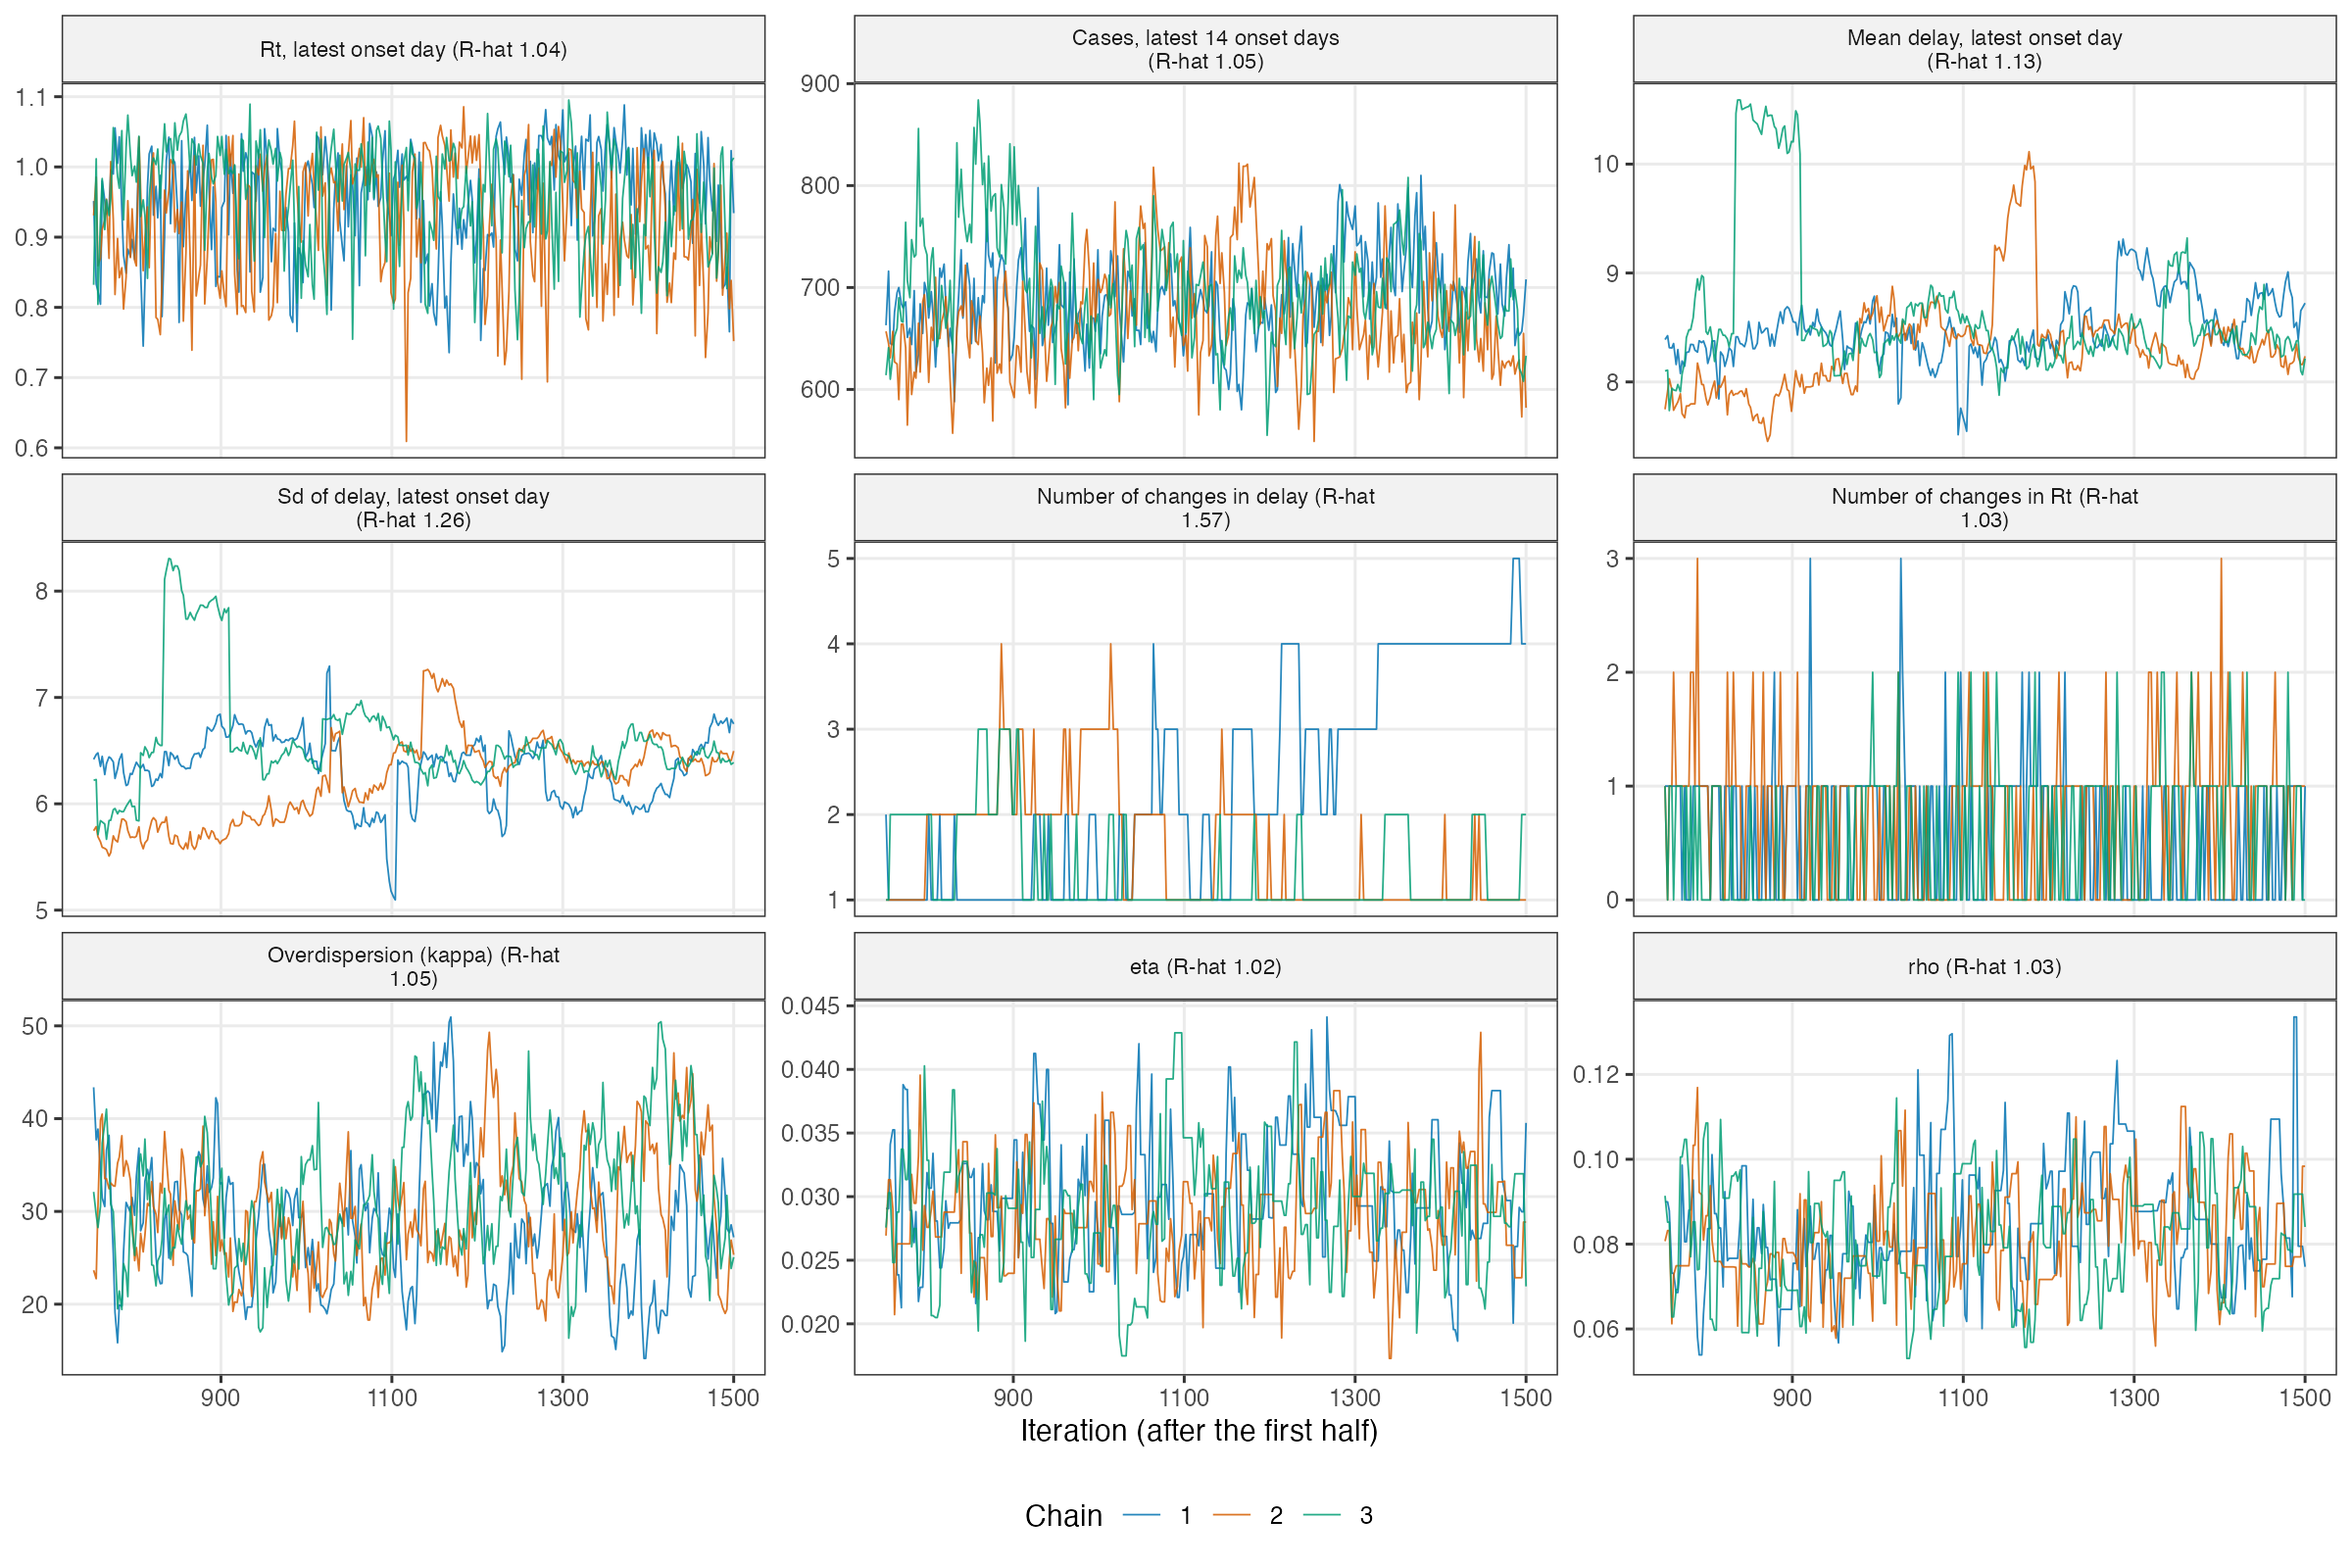
\includegraphics[width=\textwidth]{bvd_changepoint_convergence.png}
\caption{Traces of the three chains for the analysis of 1 October, after the
first half of each chain.}
\label{fig:convergence}
\end{figure}

\begin{itemize}[itemsep=2pt]
\item \emph{The quantities of most interest have converged.} For $R_t$, for
the estimated cases of every onset day, for the number of changes in $R_t$
and for $\eta$ and $\rho$, $\widehat R$ is at most 1.05 on every date but one
(1.10 for one onset day on 20 September), and the three chains, started from
different values, give the same answers.
\item \emph{The reporting delay has not.} The chains differ in the number of
changes in the delay which they visit ($\widehat R$ up to 1.57): in the
analysis of 1 October one chain moves steadily towards four or five changes
while the other two stay at one or two (figure~\ref{fig:convergence}). The
mean and standard deviation of the delay, and on some dates the effects of
the day of the week, inherit this. Proposing splits and merges five times an
iteration has made moves between configurations much more frequent than in
the single chain run before, but not frequent enough.
\item \emph{This does not appear to affect the estimates of cases or $R_t$},
which agree between chains whatever configuration of the delay each is in.
The delays in the different configurations are similar (means between about
8 and 9 days), which is presumably why. But statements about how many times
the delay changed, and when, should not be made from these runs.
\end{itemize}

\section{Limitations}

\begin{itemize}[itemsep=2pt]
\item \emph{Convergence for the reporting delay}, as just described. Longer
chains, or better moves between configurations of the delay, are needed
before the changes in the delay can be reported. A simpler alternative is a
single delay throughout, which the estimates of recent cases here suggest
would give much the same answers.
\item \emph{The serial interval} is that of Zaire ebolavirus, cut off at 40
days.
\item \emph{Cases before 12 July} are taken to be known exactly from the
report of the analysis date. For analyses dated before 6 September these
include 119 cases later removed.
\item \emph{Changes close to the analysis date.} In simulation, a change in
the delay or in $R_t$ in the week before the analysis date is not reliably
told from a change in incidence. The estimates for the latest onset days
assume, in effect, that reporting has continued as in recent weeks.
\end{itemize}

\begin{thebibliography}{6}

\bibitem{bajaj2025}
Bajaj S, Thompson R, Lambert B. 2025
A renewal-equation approach to estimating $R_t$ and infectious disease case
counts in the presence of reporting delays.
\emph{Phil. Trans. R. Soc. A} \textbf{383}, 20240357.
\href{https://doi.org/10.1098/rsta.2024.0357}{doi:10.1098/rsta.2024.0357}

\bibitem{creswell2022}
Creswell R, Robinson M, Gavaghan D, Parag KV, Lei CL, Lambert B. A Bayesian
nonparametric method for detecting rapid changes in disease transmission.
\emph{medRxiv} 2022.
\href{https://doi.org/10.1101/2022.07.04.22277234}{doi:10.1101/2022.07.04.22277234}.

\bibitem{barry1992}
Barry D, Hartigan JA. 1992
Product partition models for change point problems.
\emph{Ann. Stat.} \textbf{20}, 260--279.

\bibitem{barry1993}
Barry D, Hartigan JA. 1993
A Bayesian analysis for change point problems.
\emph{J. Am. Stat. Assoc.} \textbf{88}, 309--319.

\bibitem{cori2013}
Cori A, Ferguson NM, Fraser C, Cauchemez S. 2013
A new framework and software to estimate time-varying reproduction numbers
during epidemics.
\emph{Am. J. Epidemiol.} \textbf{178}, 1505--1512.

\bibitem{who2014}
WHO Ebola Response Team. 2014
Ebola virus disease in West Africa---the first 9 months of the epidemic and
forward projections.
\emph{N. Engl. J. Med.} \textbf{371}, 1481--1495.
\end{thebibliography}

\end{document}
